\chapter{Cochabamba et le parc de Torotoro}
\section*{28 avril 2015}
Départ de Sucre direction Cochabamba. Beaucoup de descente le premier jour, les températures deviennent plus élevées. \newline
 \newline
\centerline{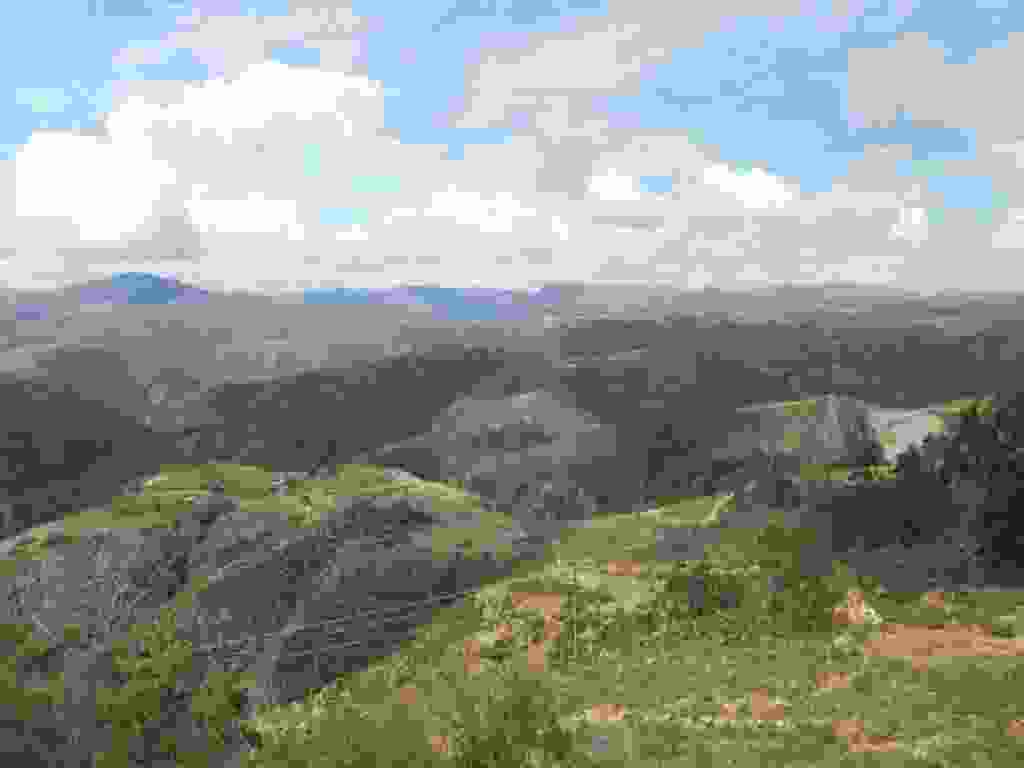
\includegraphics[height=90mm]{../wp-content/uploads/2015/04/wpid-wp-1429714724768-1024x768.jpg} } 
 \newline
 \newline
\centerline{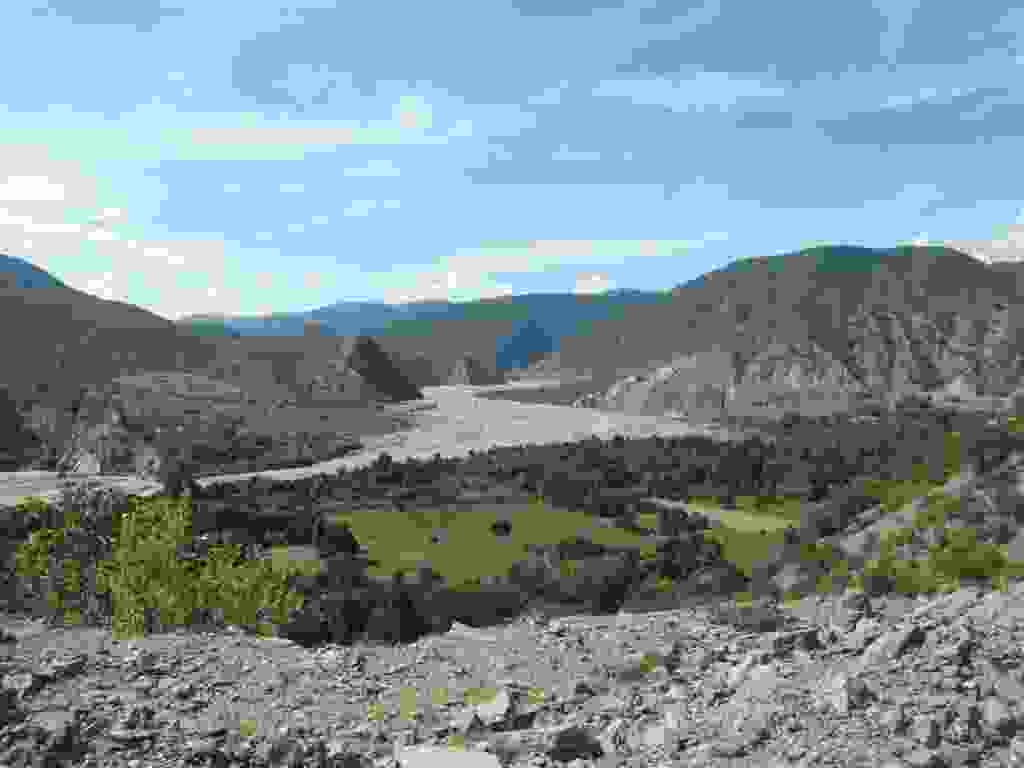
\includegraphics[height=90mm]{../wp-content/uploads/2015/04/wpid-wp-1429714753090-1024x768.jpg} } 
 \newline
 \newline
\centerline{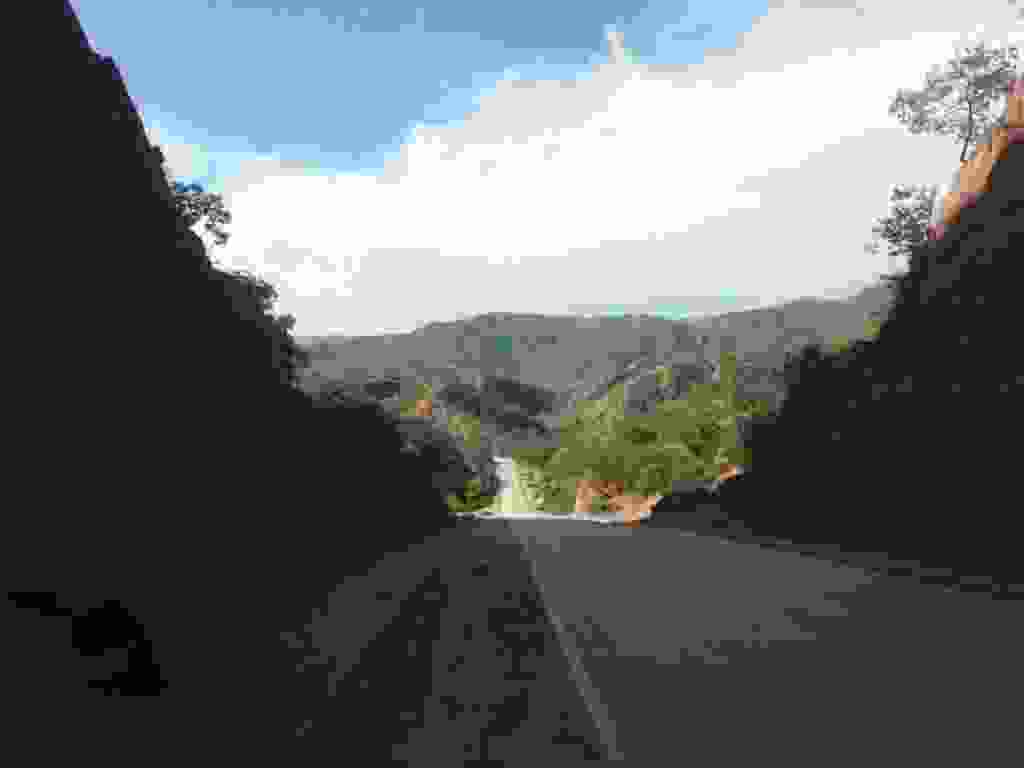
\includegraphics[height=90mm]{../wp-content/uploads/2015/04/wpid-wp-1429714770711-1024x768.jpg} } 
 \newline
 Premier bivouac où il a fait très chaud et avec la compagnie des moustiques. \newline
 \newline
\centerline{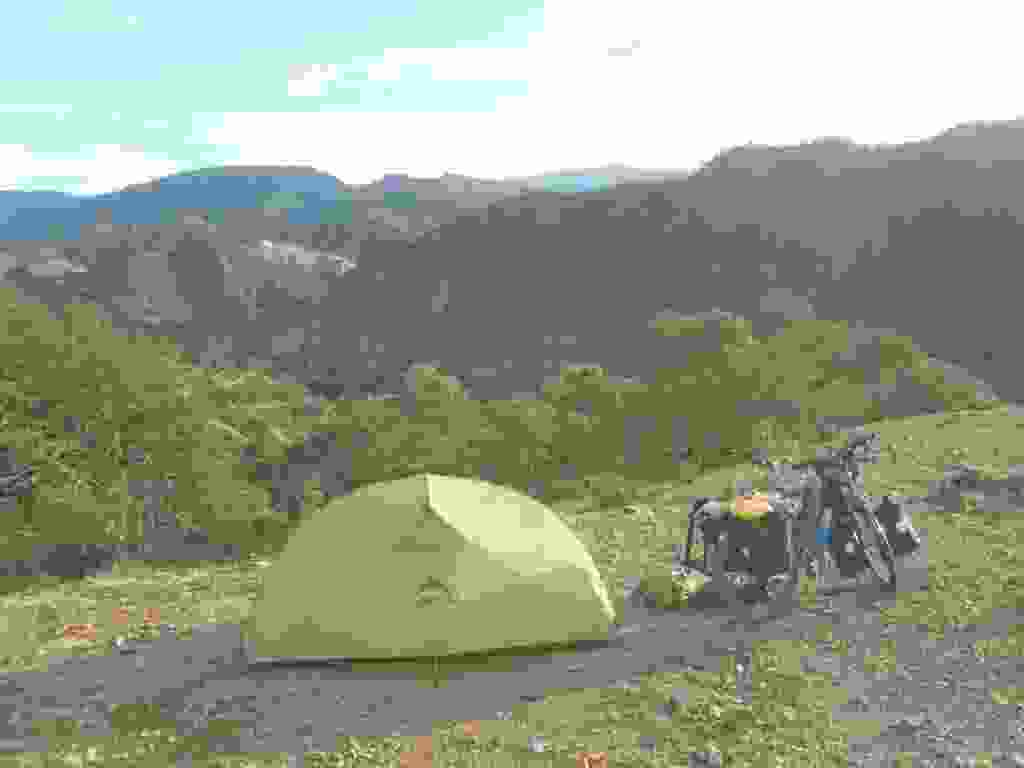
\includegraphics[height=90mm]{../wp-content/uploads/2015/04/wpid-wp-1429714848743-1024x768.jpg} } 
 \newline
 En traversant un village le lendemain, je suis arrêté par un homme qui me dit qu'il est le chef du village. \newline
 \newline
\centerline{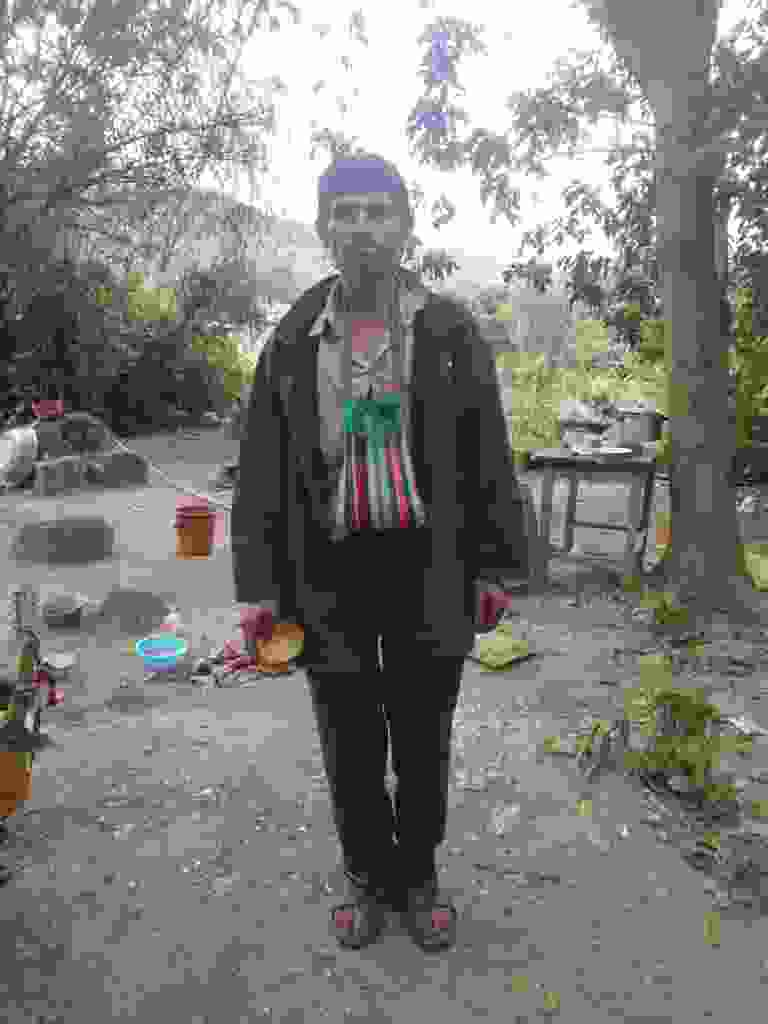
\includegraphics[height=90mm]{../wp-content/uploads/2015/04/wpid-wp-1429715140310-768x1024.jpg} } 
 \newline
 Il m'invite à boire un coup avec ses amis, manifestement ils n'en sont pas au premier verre. \newline
 \newline
\centerline{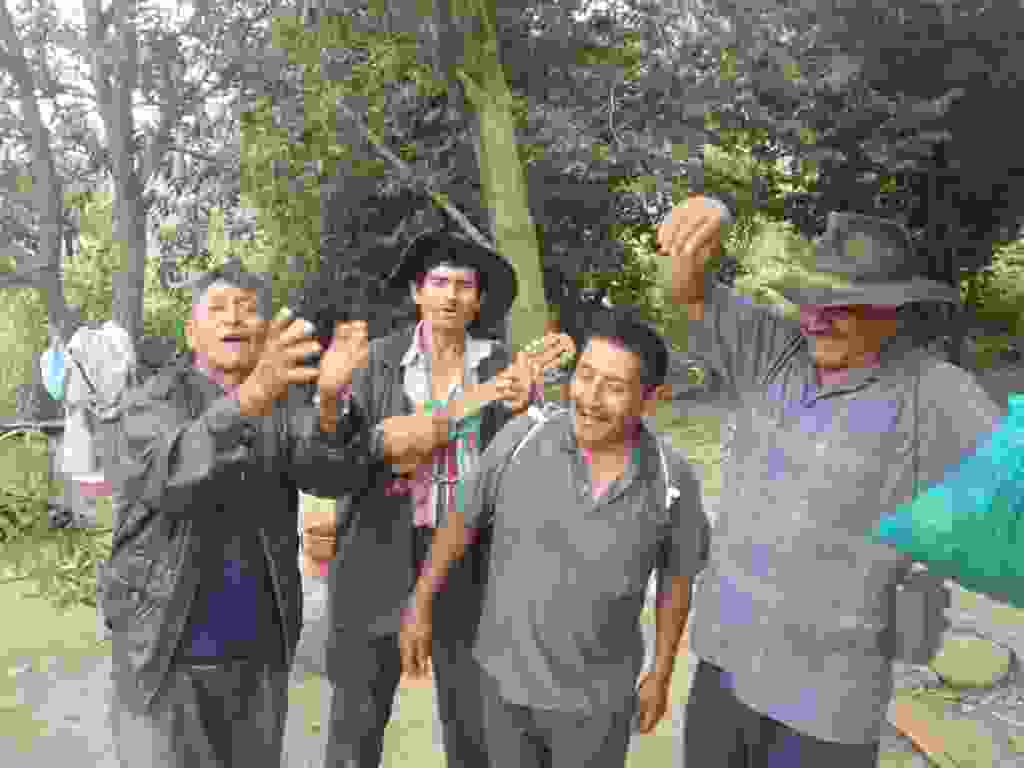
\includegraphics[height=90mm]{../wp-content/uploads/2015/04/wpid-wp-1429715261110-1024x768.jpg} } 
 \newline
 Puis j'arrive à Aiquile, la capitale du Charango la mini guitare sur la photo précédente. \newline
 \newline
\centerline{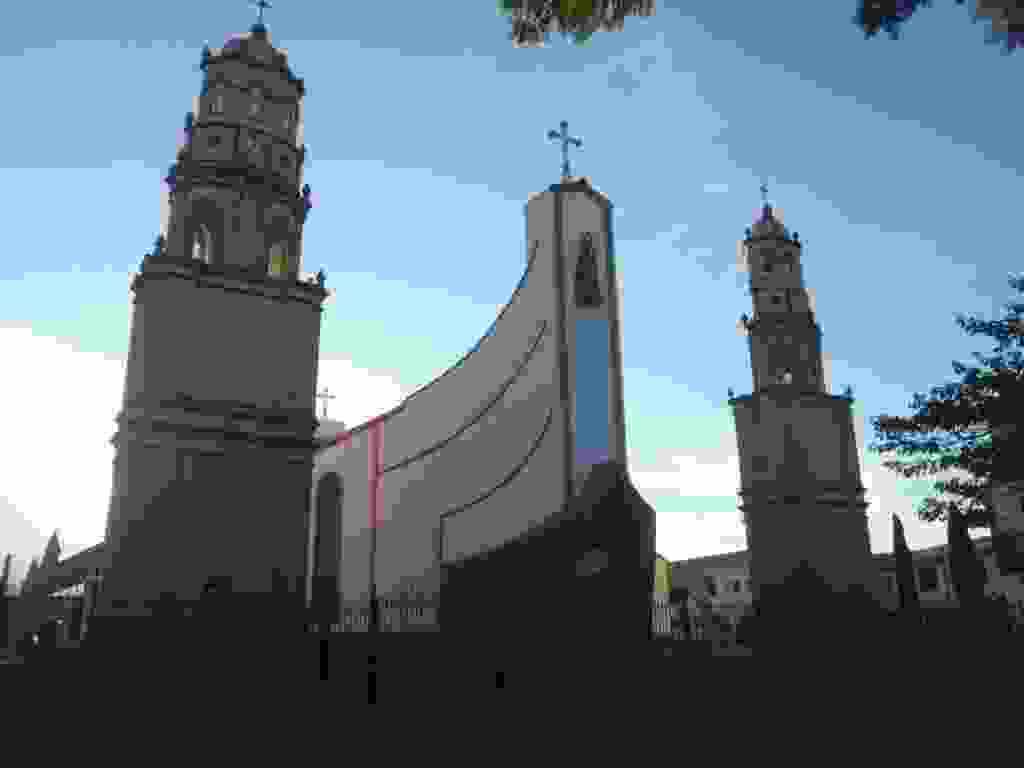
\includegraphics[height=90mm]{../wp-content/uploads/2015/04/wpid-wp-1429715491596-1024x768.jpg} } 
 \newline
 Je rencontre un nouveau type de route en pierre : pas très agréable ça secoue beaucoup. \newline
 \newline
\centerline{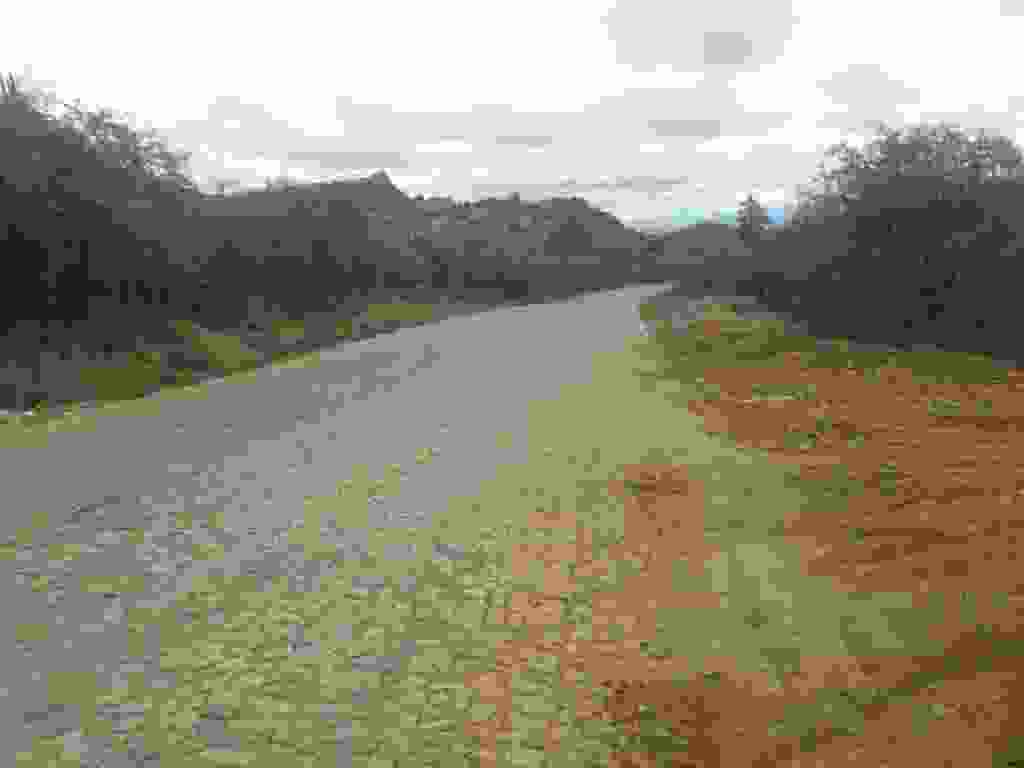
\includegraphics[height=90mm]{../wp-content/uploads/2015/04/wpid-wp-1429716153838-1024x768.jpg} } 
 \newline
 Le bord est plus roulant mais cette route est bordée d'arbustes avec des épines vraiment grandes. Au bout de 10km c'est la première crevaison du voyage. Je répare et en remontant c'est l'attache de la roue arrière qui casse. \newline
 Pas le choix je dois faire du stop, un camion s'arrête assez rapidement et par chance il va vers Cochabamba. C'est parti pour 200km à l'arrière du camion ! \newline
 \newline
\centerline{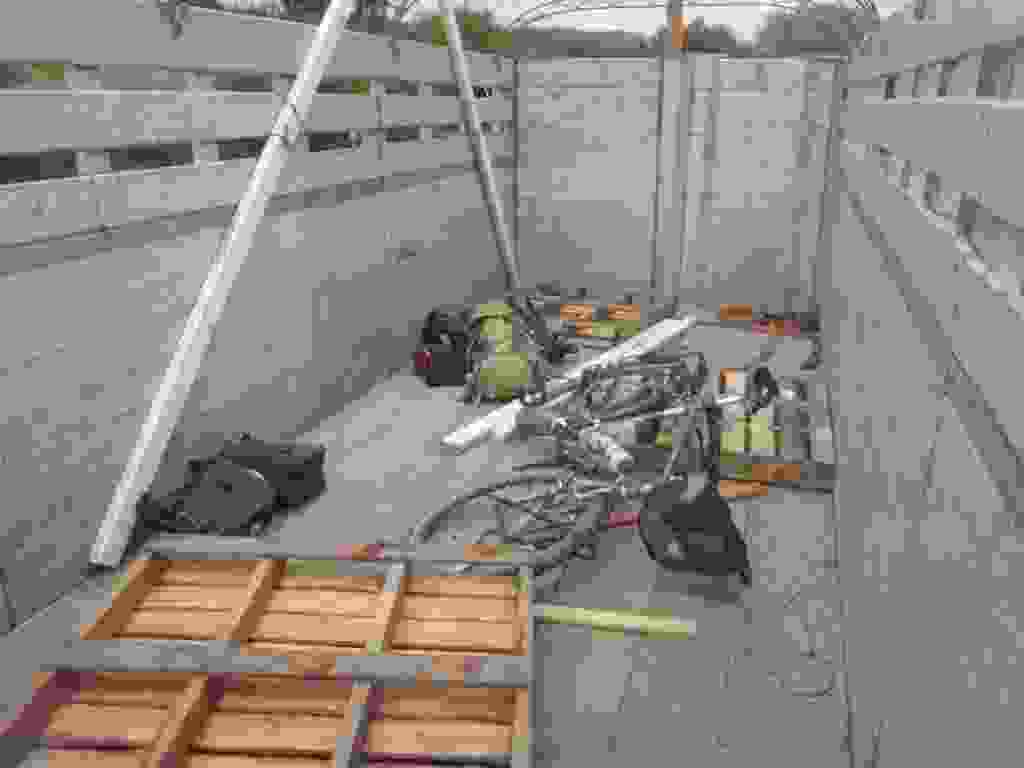
\includegraphics[height=90mm]{../wp-content/uploads/2015/04/wpid-wp-1429716662010-1024x768.jpg} } 
 \newline
 Je rate une belle portion de route à flan de montagne mais cela m´évite aussi de longues montées sur une surface difficile. \newline
 \newline
\centerline{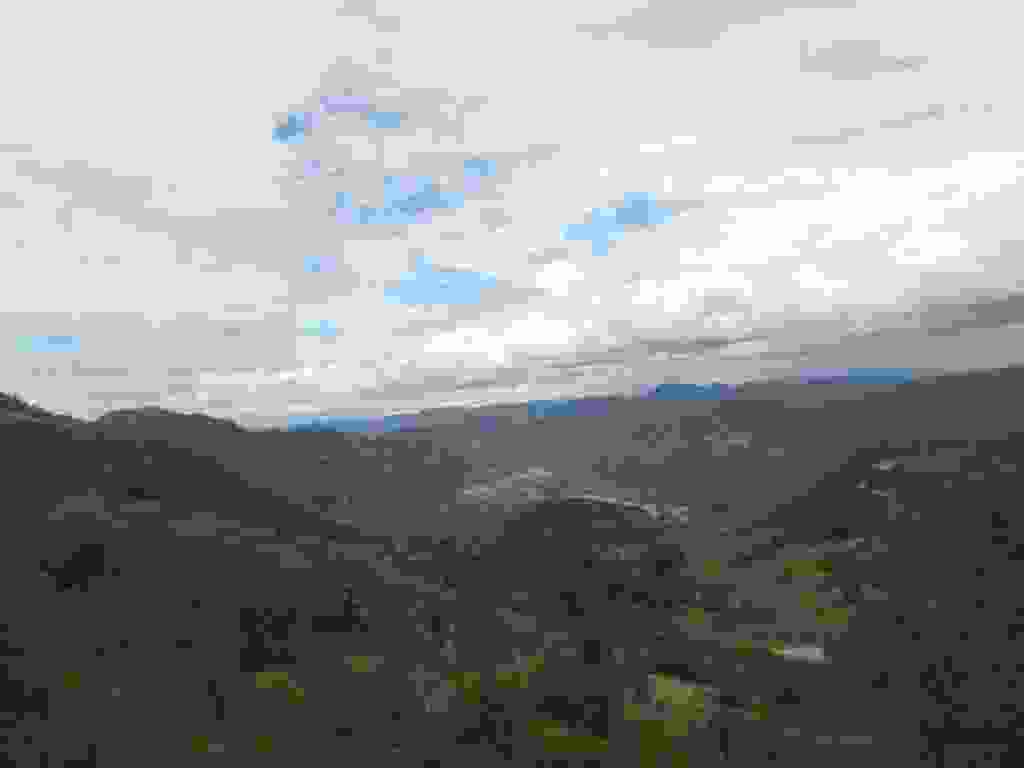
\includegraphics[height=90mm]{../wp-content/uploads/2015/04/wpid-wp-1429717092474-1024x768.jpg} } 
 \newline
 \newline
\centerline{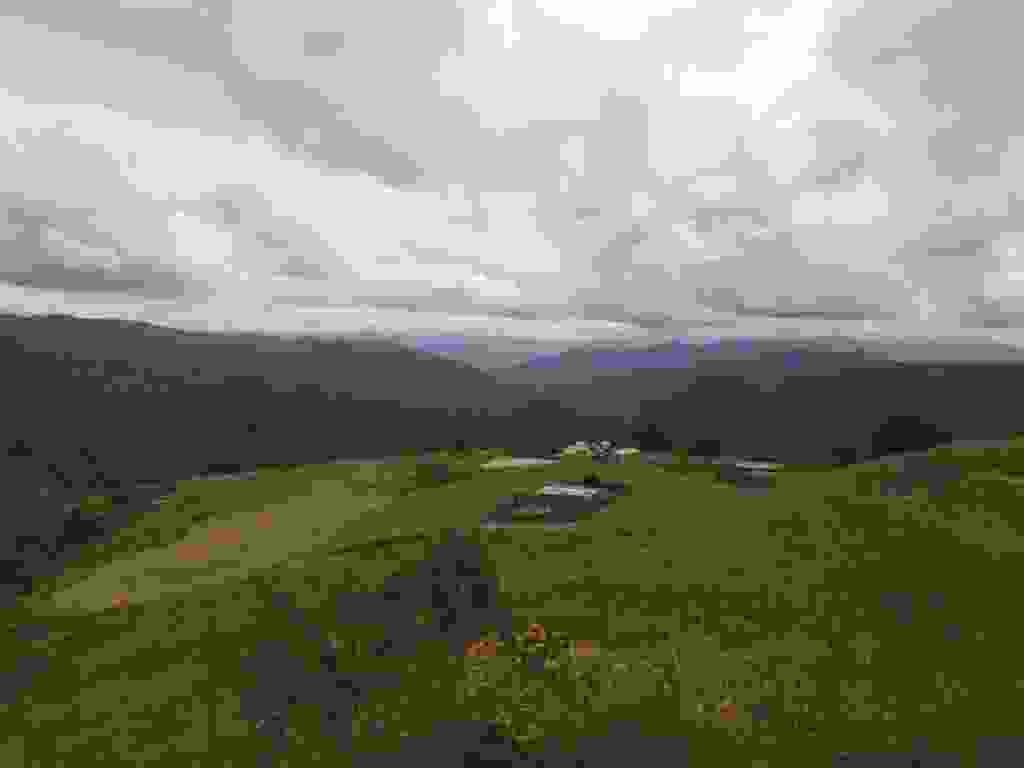
\includegraphics[height=90mm]{../wp-content/uploads/2015/04/wpid-wp-1429717103661-1024x768.jpg} } 
 \newline
 Du coup j'arrive plus vite que prévu à Cochabamba où je suis hébergé par Hache, américain de 75 ans qui a voyagé en vélo de nombreuses années. \newline
 \newline
\centerline{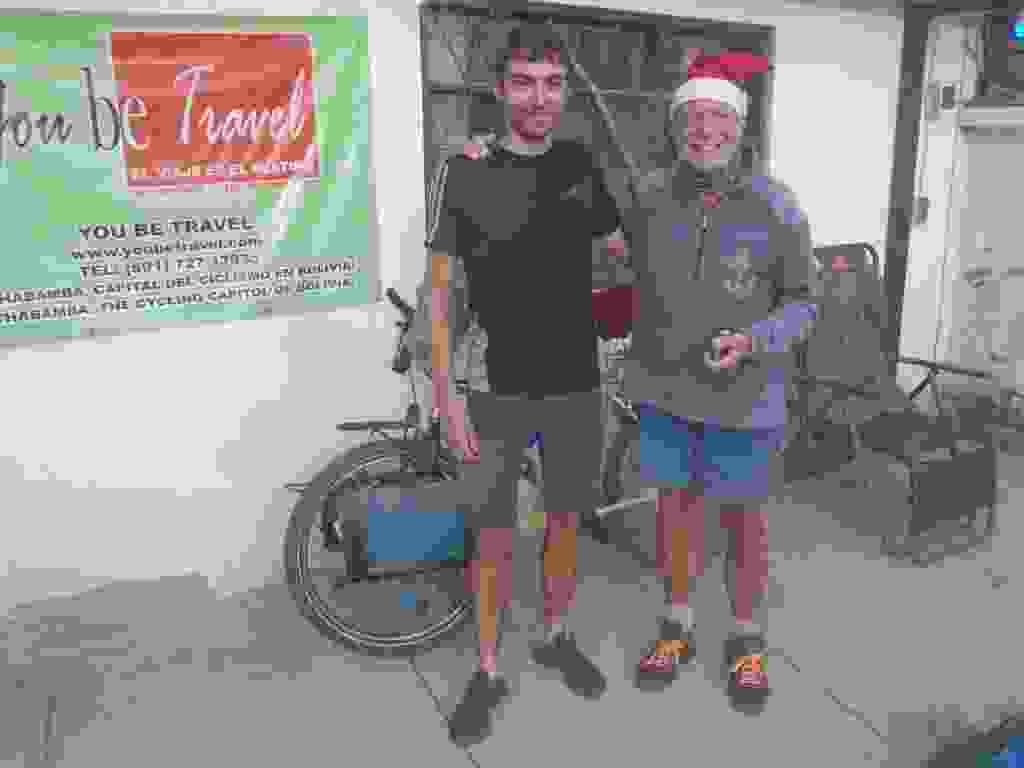
\includegraphics[height=90mm]{../wp-content/uploads/2015/04/wpid-wp-1430169754284-1024x768.jpg} } 
 \newline
 Je rencontre aussi Johnny, cycliste argentin qui vit là. \newline
 \newline
\centerline{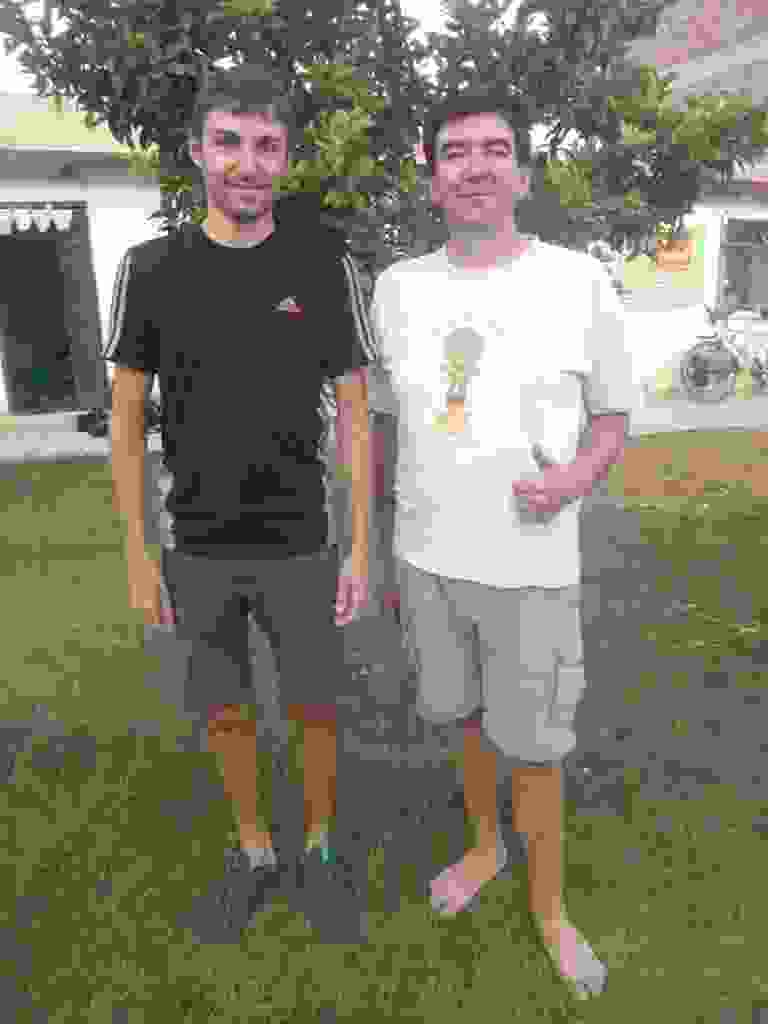
\includegraphics[height=90mm]{../wp-content/uploads/2015/04/wpid-wp-1430172032816-768x1024.jpg} } 
 \newline
 Ce très bon accueil me fait rester 1 semaine à Cochabamba qui est une ville peu touristique mais agréable. \newline
 \newline
\centerline{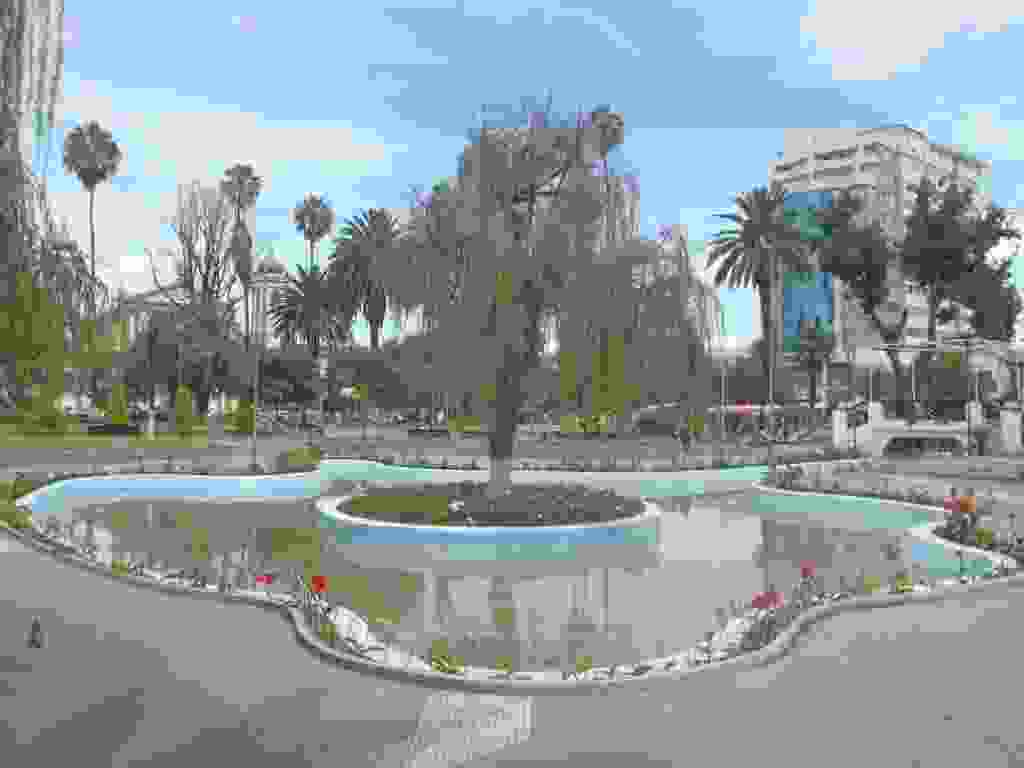
\includegraphics[height=90mm]{../wp-content/uploads/2015/04/wpid-wp-1430169894852-1024x768.jpg} } 
 \newline
 \newline
\centerline{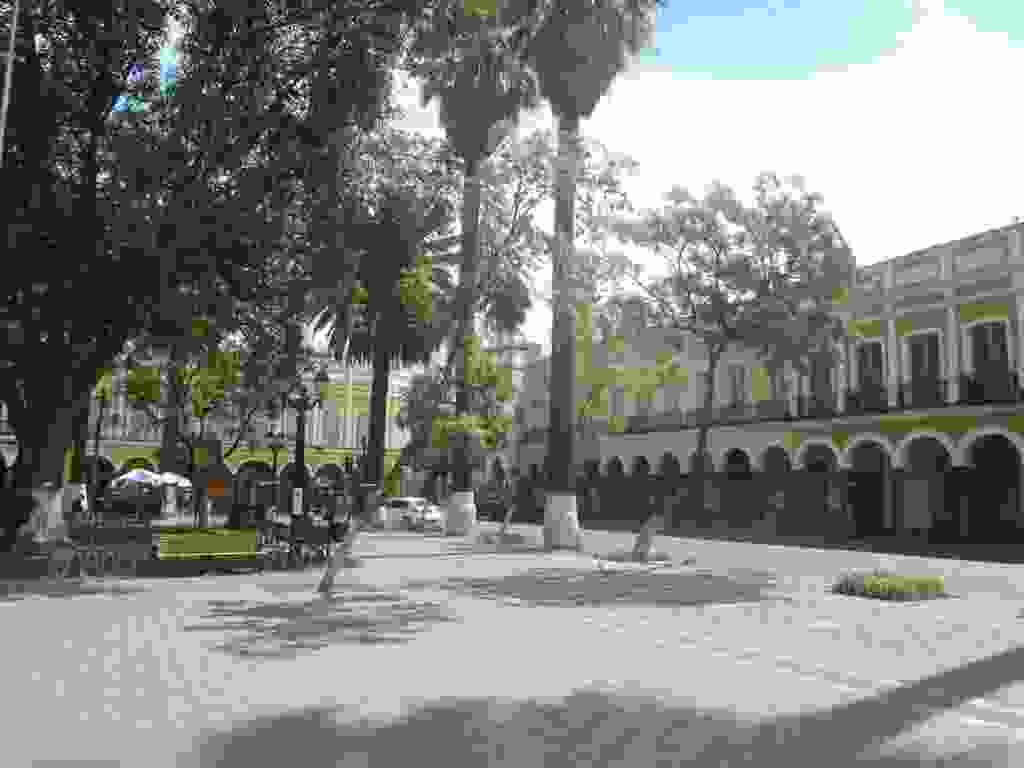
\includegraphics[height=90mm]{../wp-content/uploads/2015/04/wpid-wp-1430169968401-1024x768.jpg} } 
 \newline
 Montée au Christo de la Concordia. \newline
 \newline
\centerline{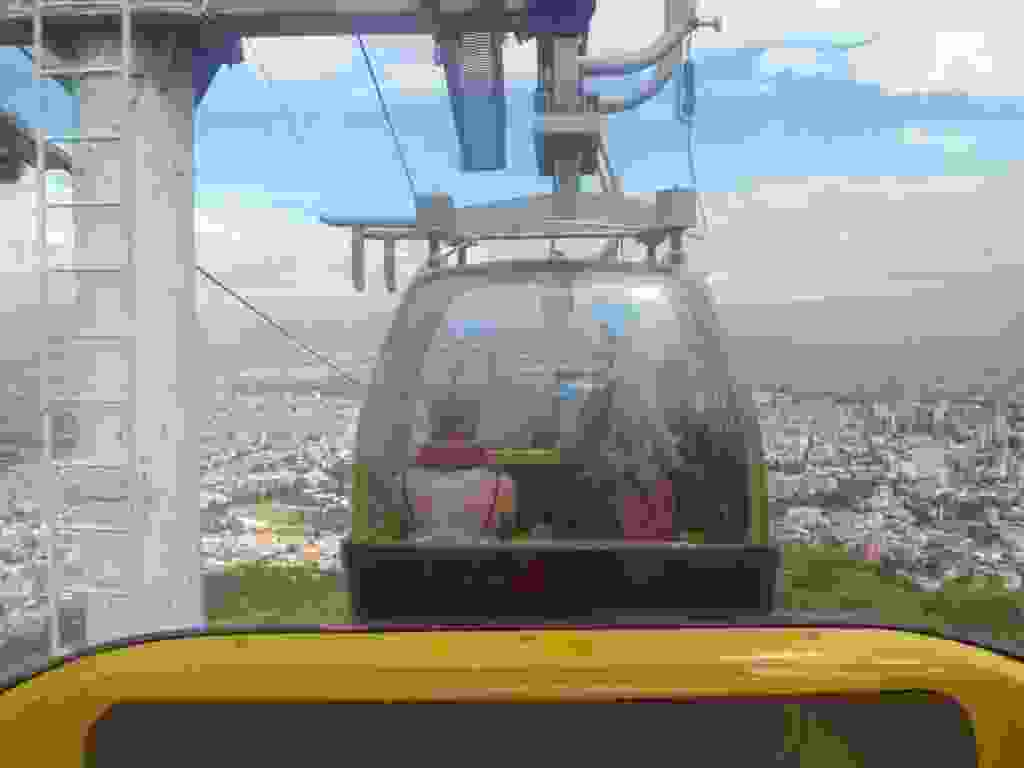
\includegraphics[height=90mm]{../wp-content/uploads/2015/04/wpid-wp-1430170103426-1024x768.jpg} } 
 \newline
 \newline
\centerline{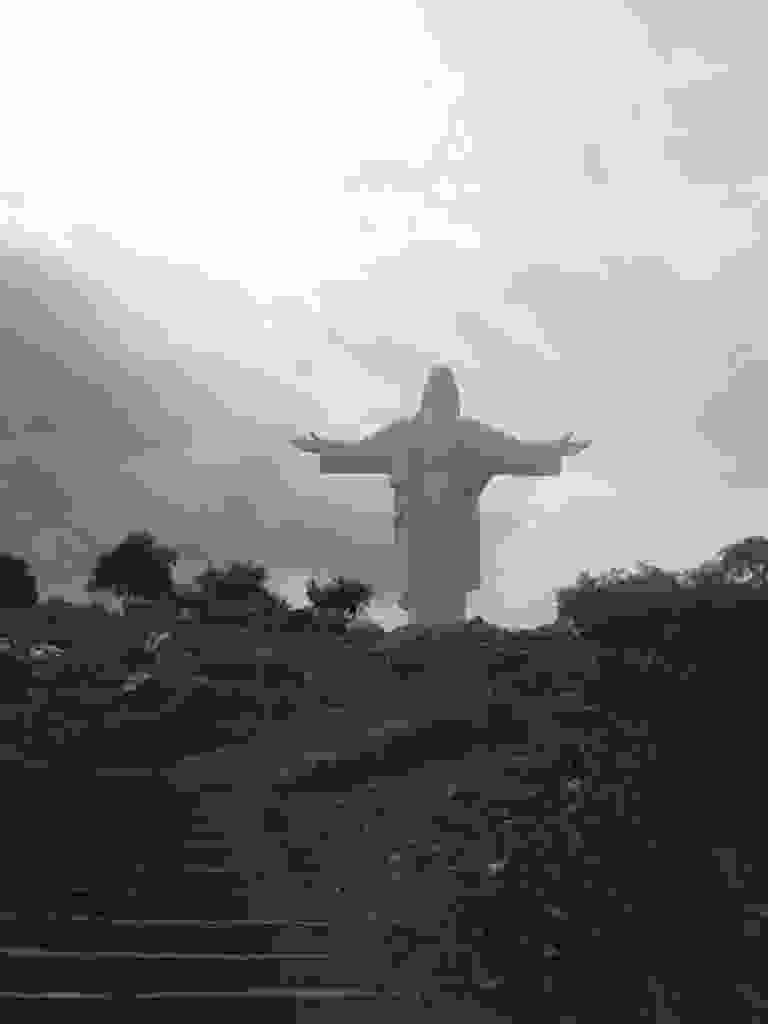
\includegraphics[height=90mm]{../wp-content/uploads/2015/04/P4213577-768x1024.jpg} } 
 \newline
 \newline
\centerline{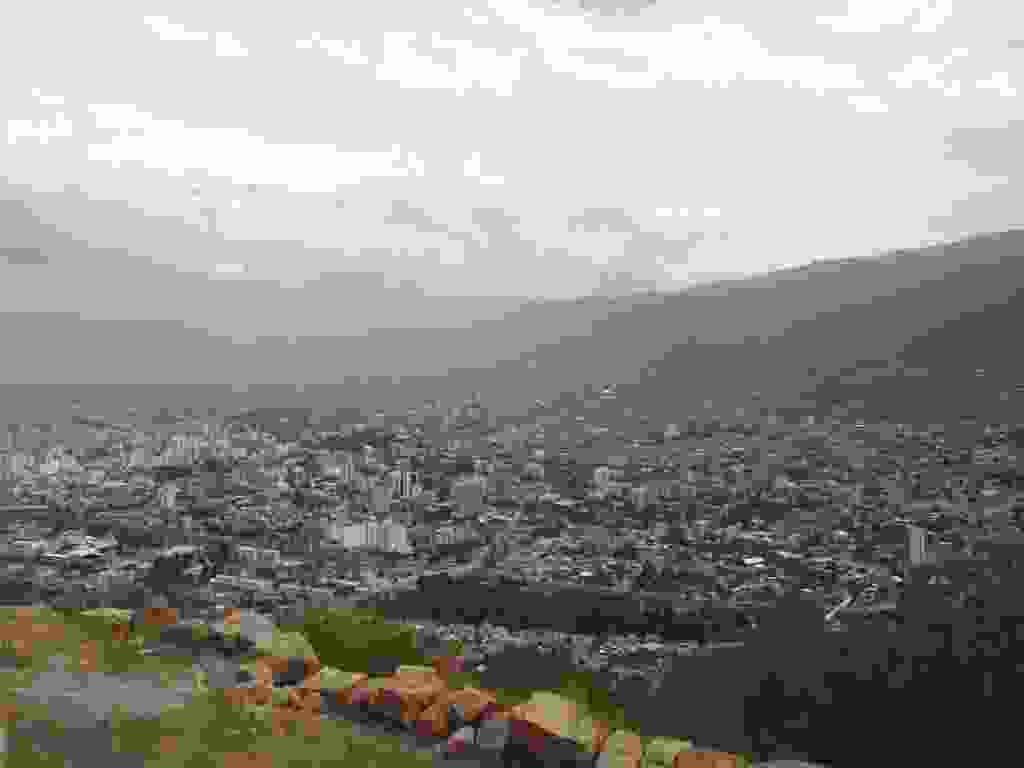
\includegraphics[height=90mm]{../wp-content/uploads/2015/04/P42135781-1024x768.jpg} } 
 \newline
 Le marché de la Cancha, immense. \newline
 \newline
\centerline{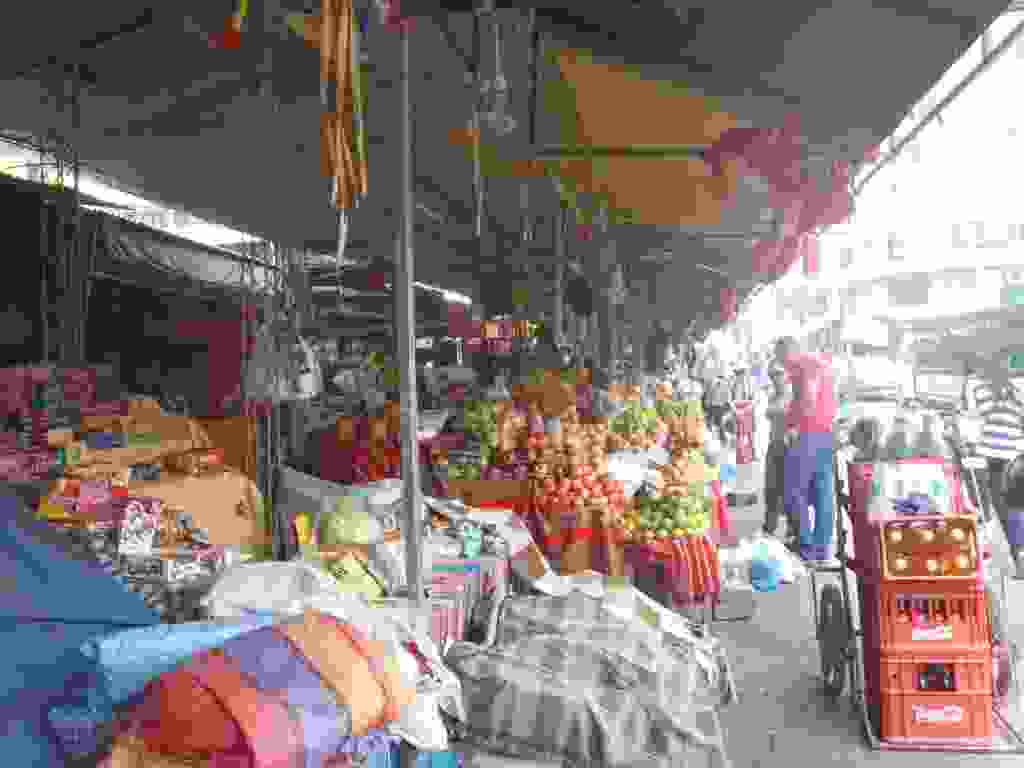
\includegraphics[height=90mm]{../wp-content/uploads/2015/04/P4213590-1024x768.jpg} } 
 \newline
 \newline
\centerline{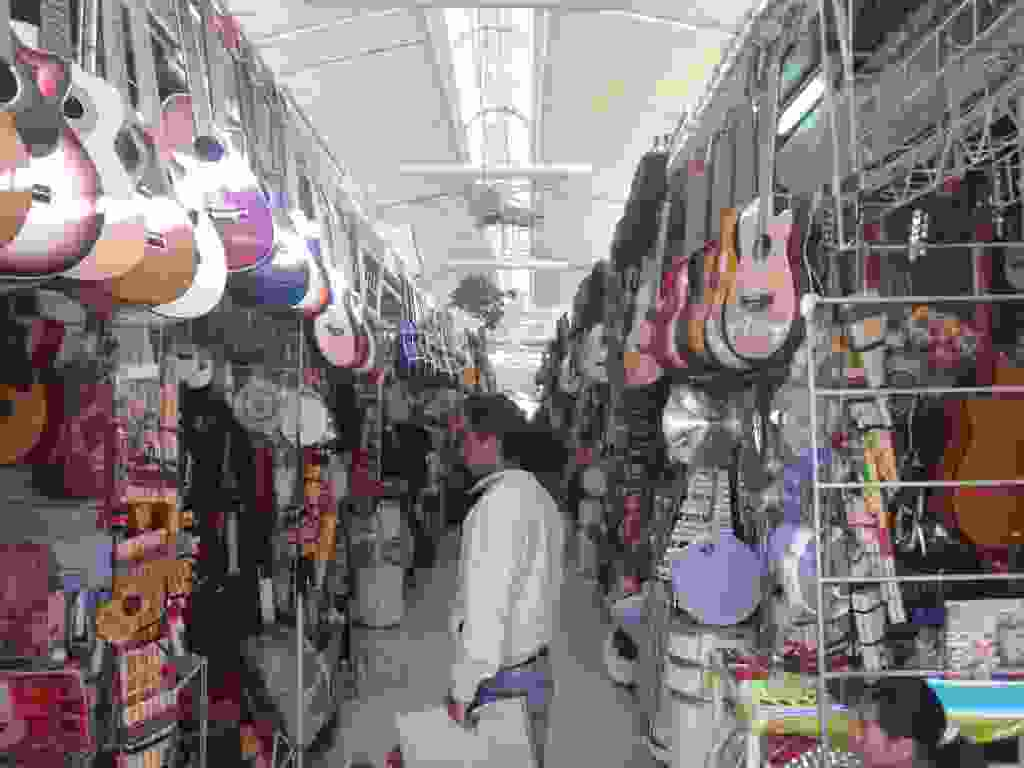
\includegraphics[height=90mm]{../wp-content/uploads/2015/04/P4213591-1024x768.jpg} } 
 \newline
 Le Palacio Portales construit par un bolivien ayant fait fortune dans le commerce de l'étain. \newline
 \newline
\centerline{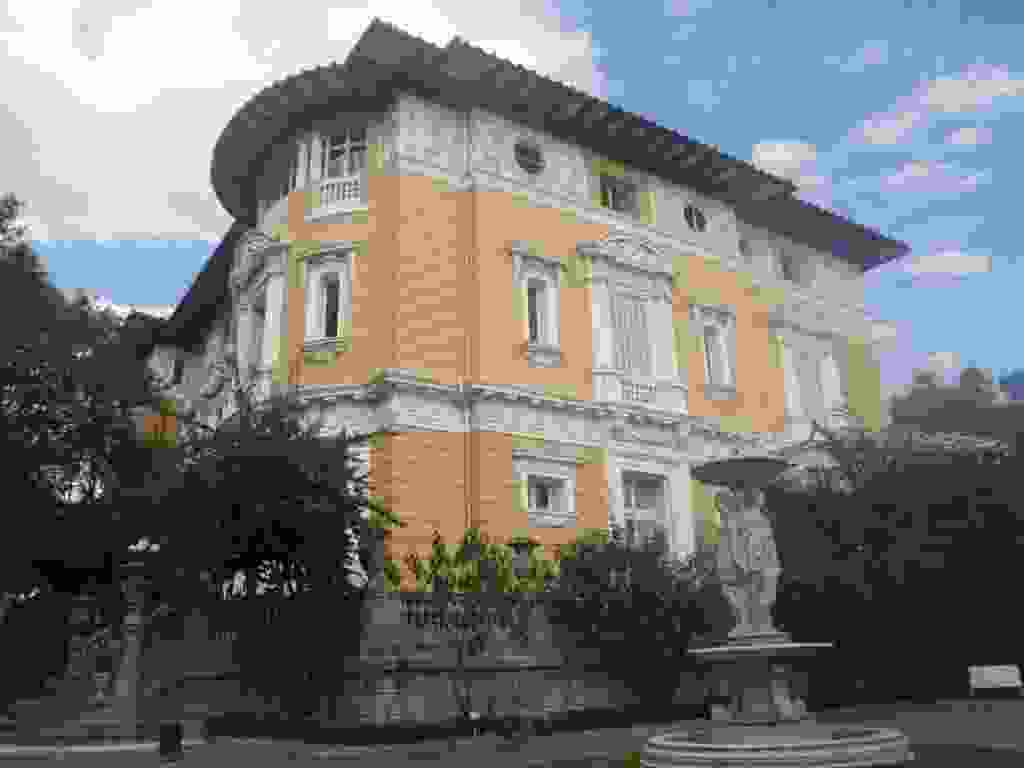
\includegraphics[height=90mm]{../wp-content/uploads/2015/04/P4213594-1024x768.jpg} } 
 \newline
 Pendant 2 jours je suis parti visiter le parc de Torotoro à 140km de Cochabamba. \newline
 \newline
\centerline{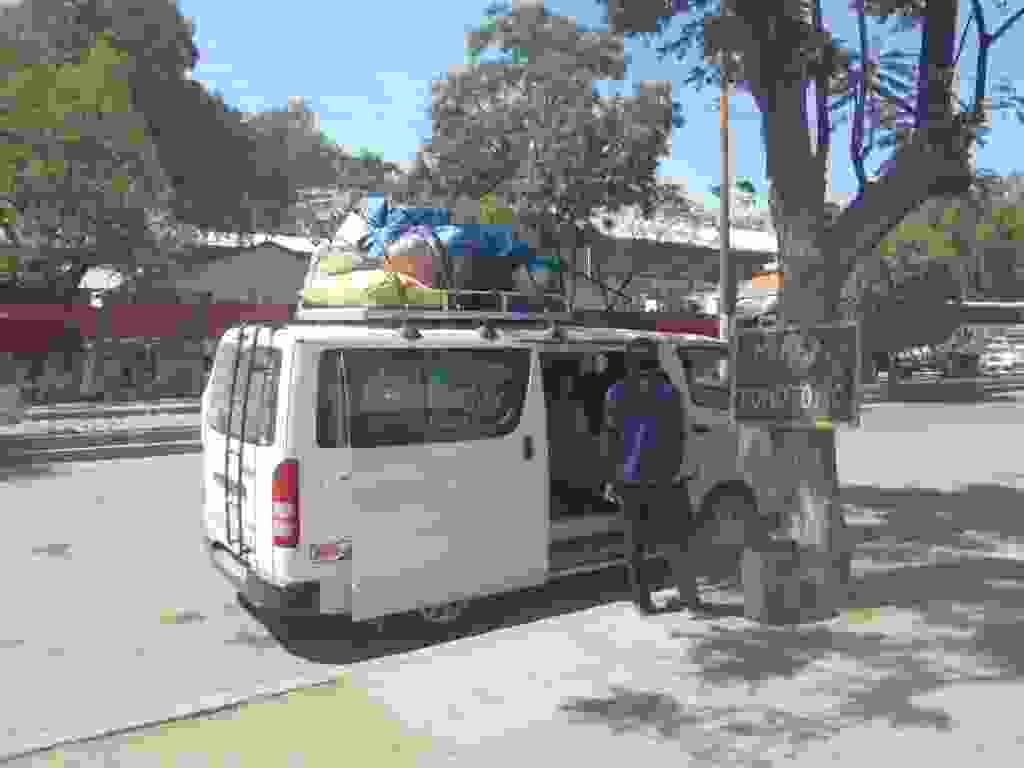
\includegraphics[height=90mm]{../wp-content/uploads/2015/04/P4243604-1024x768.jpg} } 
 \newline
 \newline
\centerline{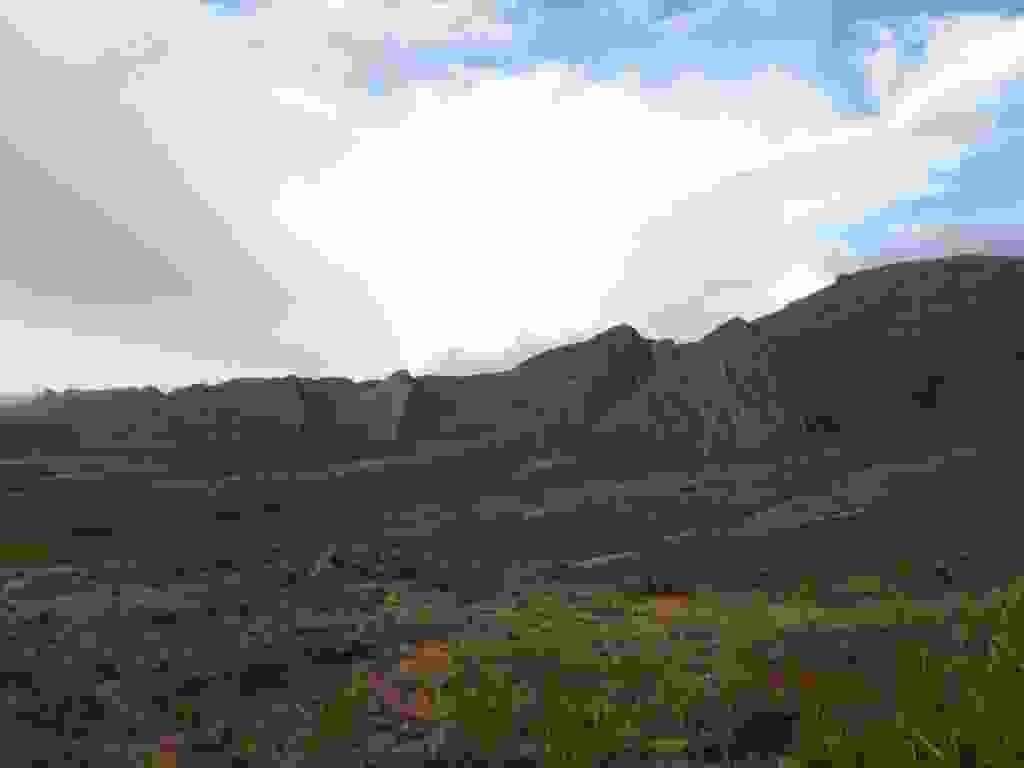
\includegraphics[height=90mm]{../wp-content/uploads/2015/04/P4253606-1024x768.jpg} } 
 \newline
 Le site de Itas : des grottes ayant été habitées pendant la préhistoire. \newline
 \newline
\centerline{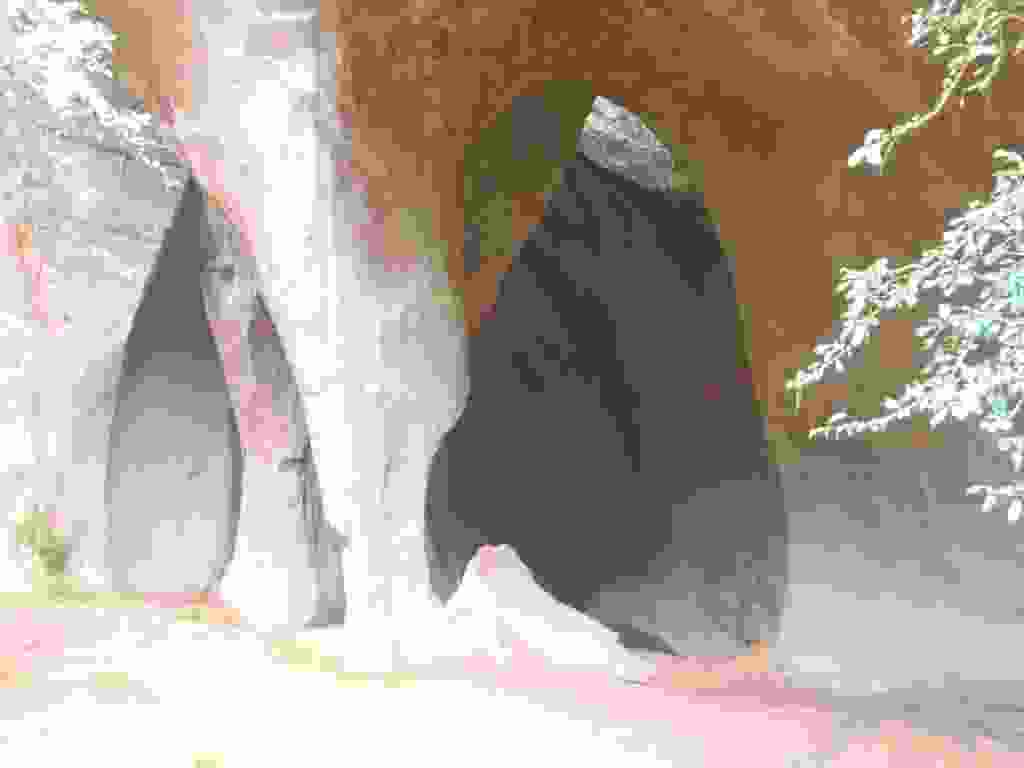
\includegraphics[height=90mm]{../wp-content/uploads/2015/04/P4253613-1024x768.jpg} } 
 \newline
 \newline
\centerline{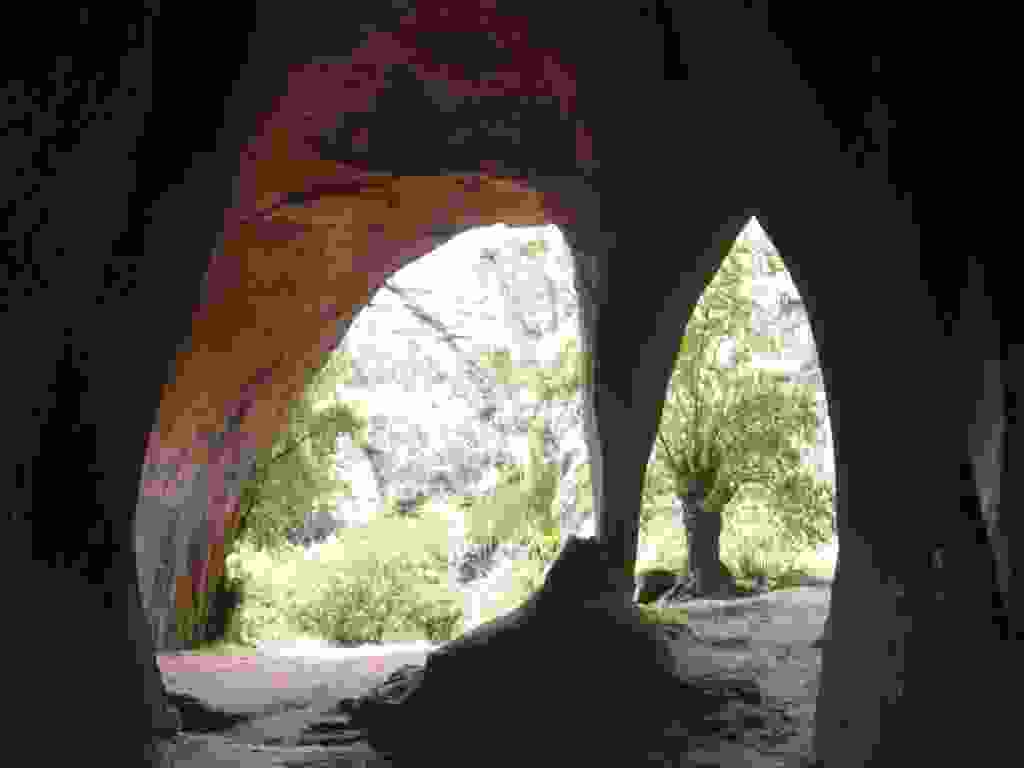
\includegraphics[height=90mm]{../wp-content/uploads/2015/04/P4253614-1024x768.jpg} } 
 \newline
 \newline
\centerline{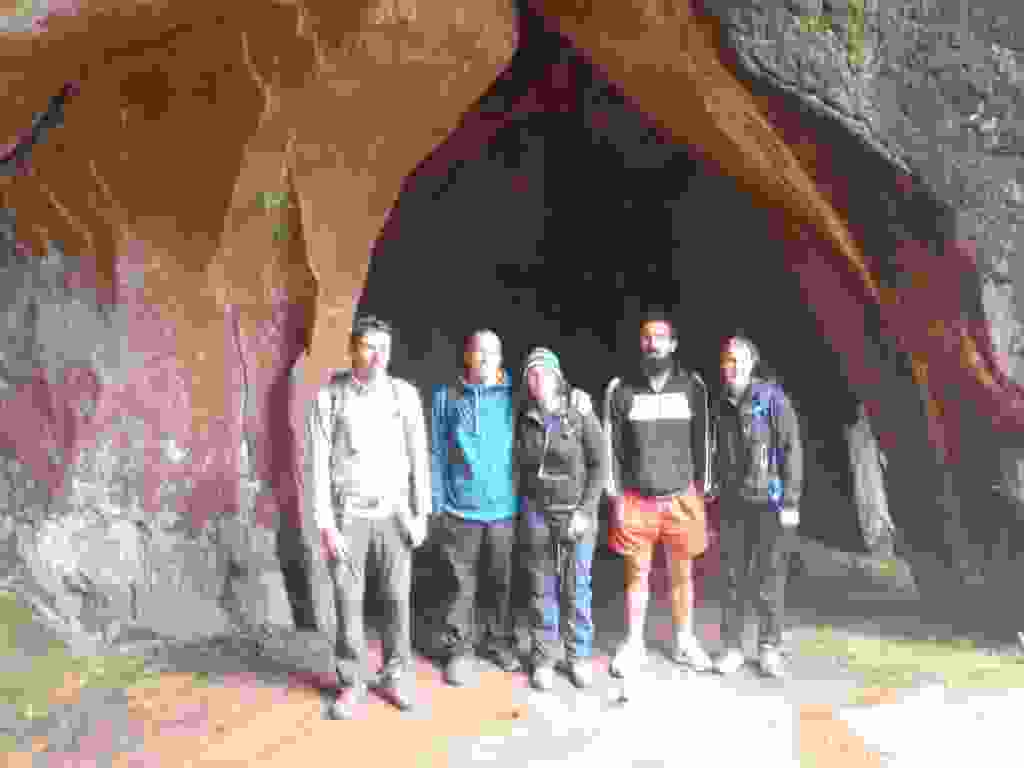
\includegraphics[height=90mm]{../wp-content/uploads/2015/04/P4253612-1024x768.jpg} } 
 \newline
 La grotte de Umajalanta : visite sportive avec des passages à plat ventre et escalades avec cordes. \newline
 \newline
\centerline{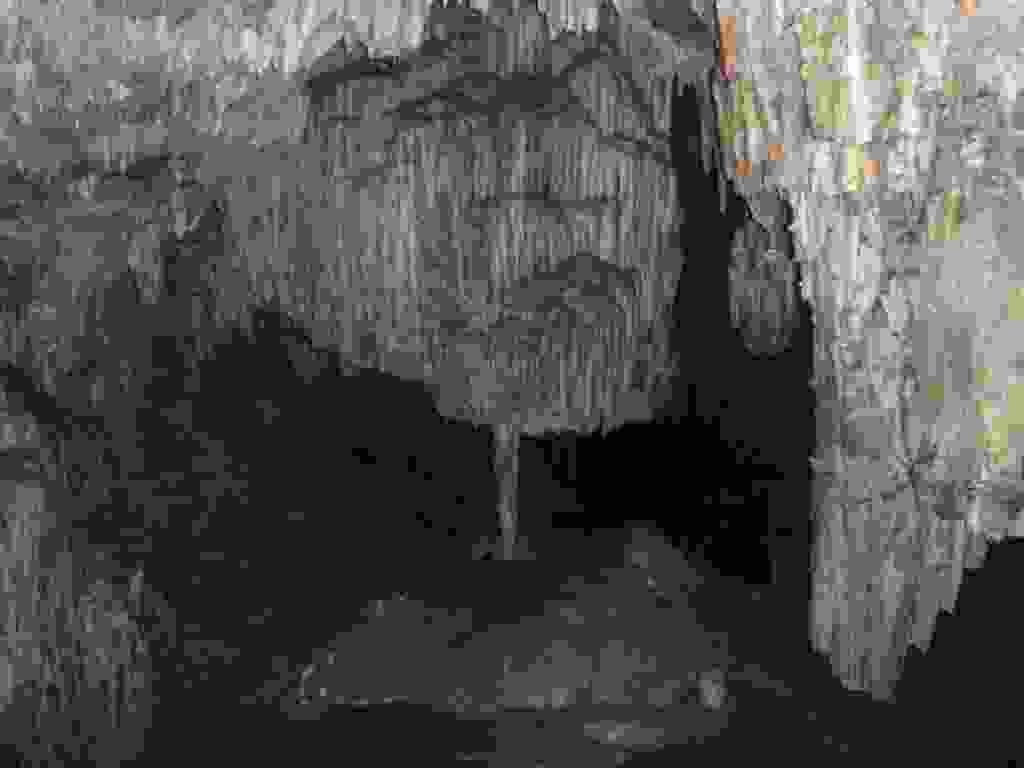
\includegraphics[height=90mm]{../wp-content/uploads/2015/04/P4253634-1024x768.jpg} } 
 \newline
 Ici pas de problème pour toucher les stalactites ou même s'y accrocher pour monter, de toute façon elles sont déjà toutes cassées. \newline
 \newline
\centerline{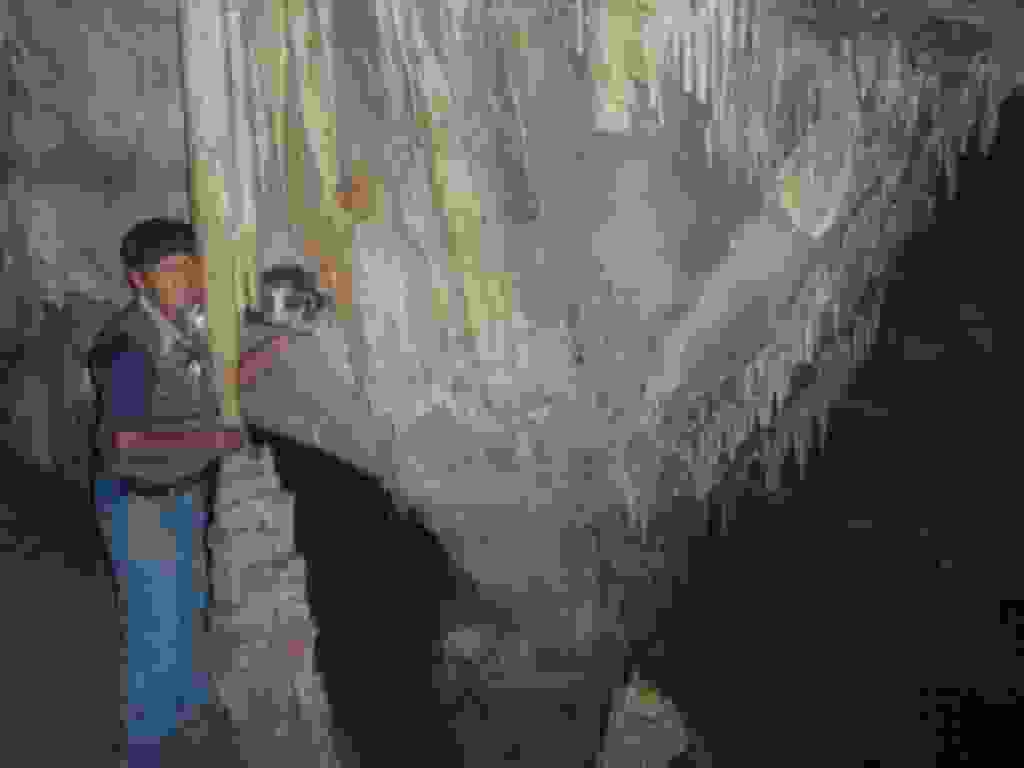
\includegraphics[height=90mm]{../wp-content/uploads/2015/04/P4253639-1024x768.jpg} } 
 \newline
 \newline
\centerline{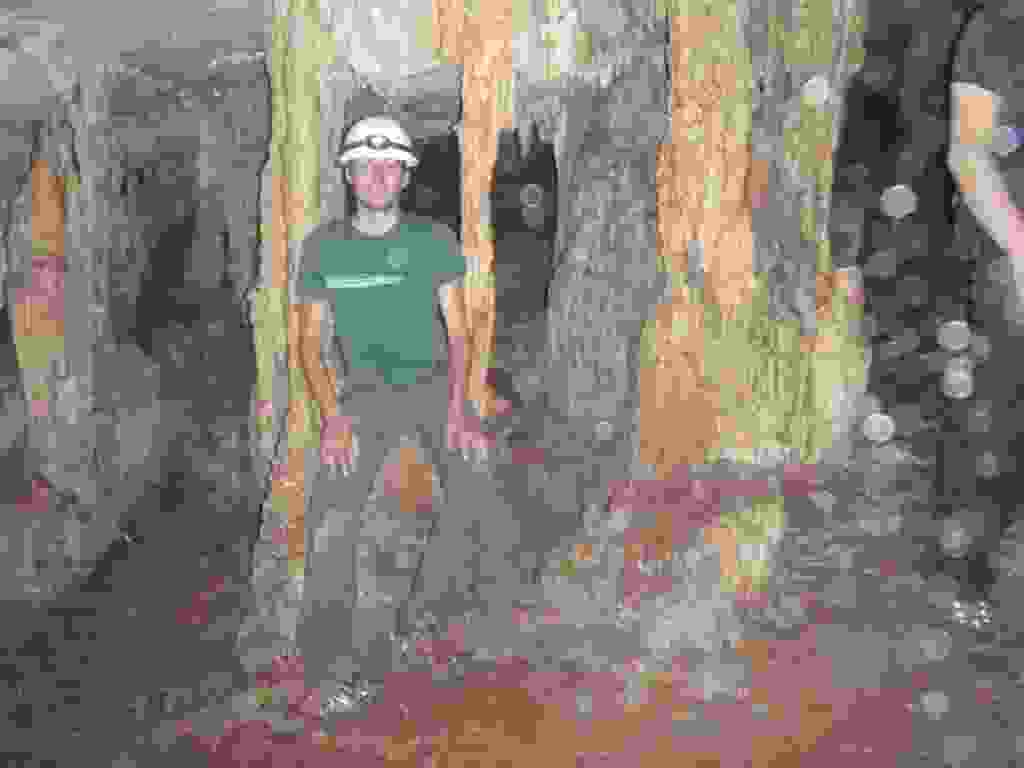
\includegraphics[height=90mm]{../wp-content/uploads/2015/04/P4253642-1024x768.jpg} } 
 \newline
 Randonnée au canyon de Vergel. \newline
 \newline
\centerline{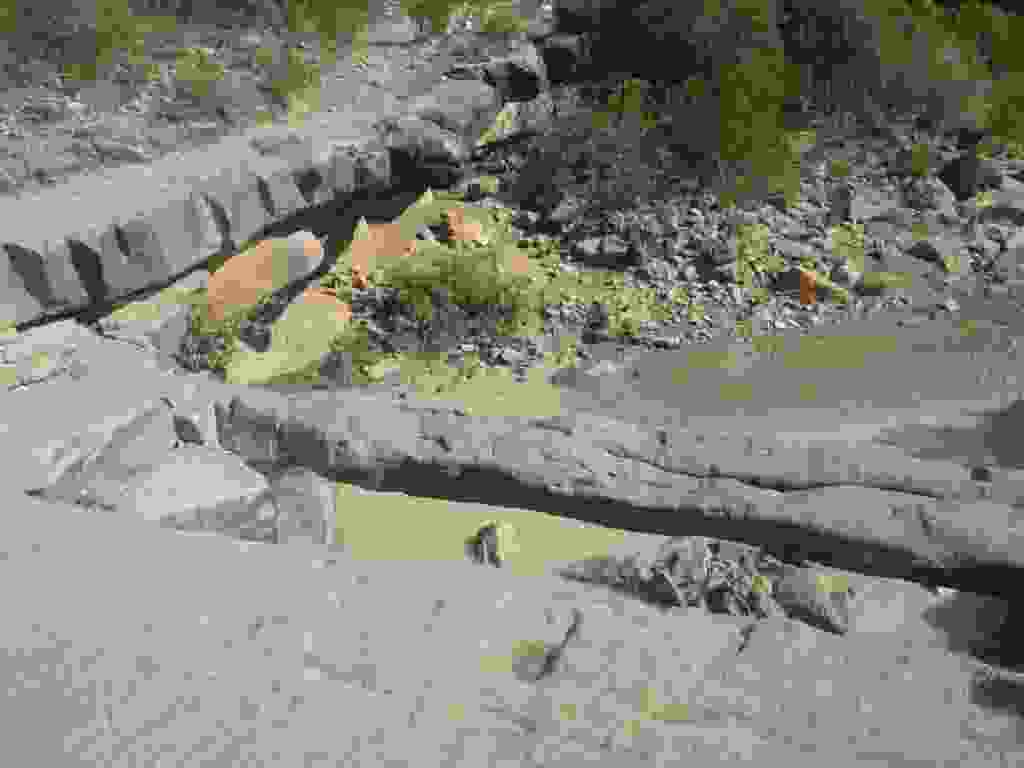
\includegraphics[height=90mm]{../wp-content/uploads/2015/04/P4263649-1024x768.jpg} } 
 \newline
 \newline
\centerline{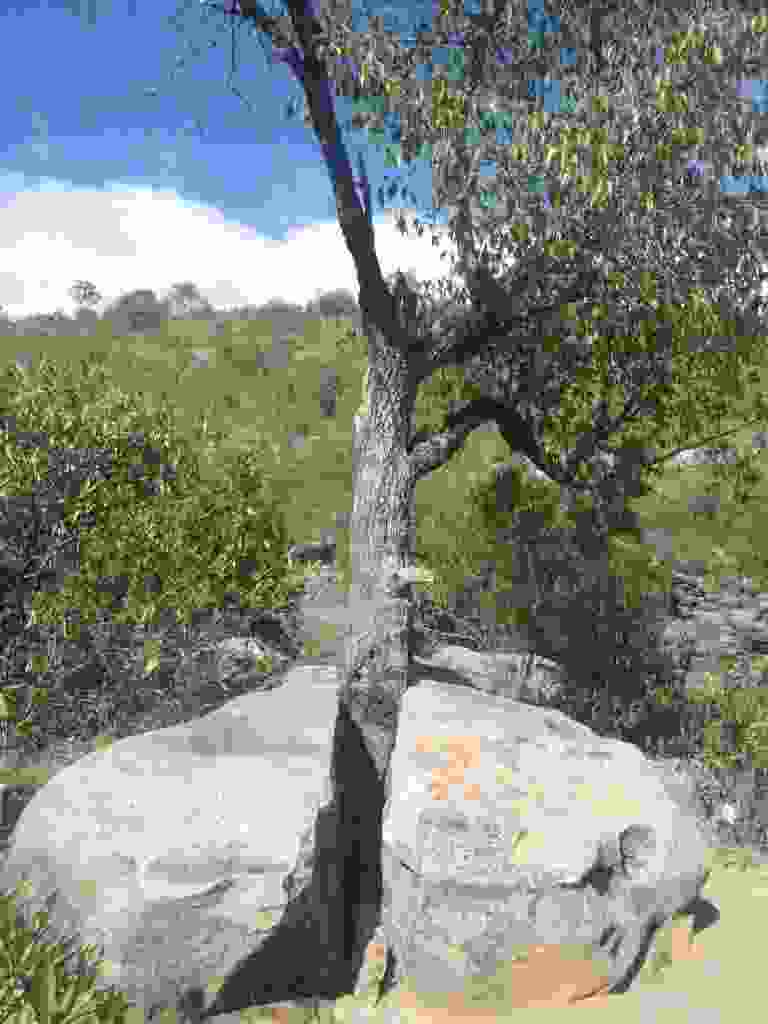
\includegraphics[height=90mm]{../wp-content/uploads/2015/04/P4263651-768x1024.jpg} } 
 \newline
 \newline
\centerline{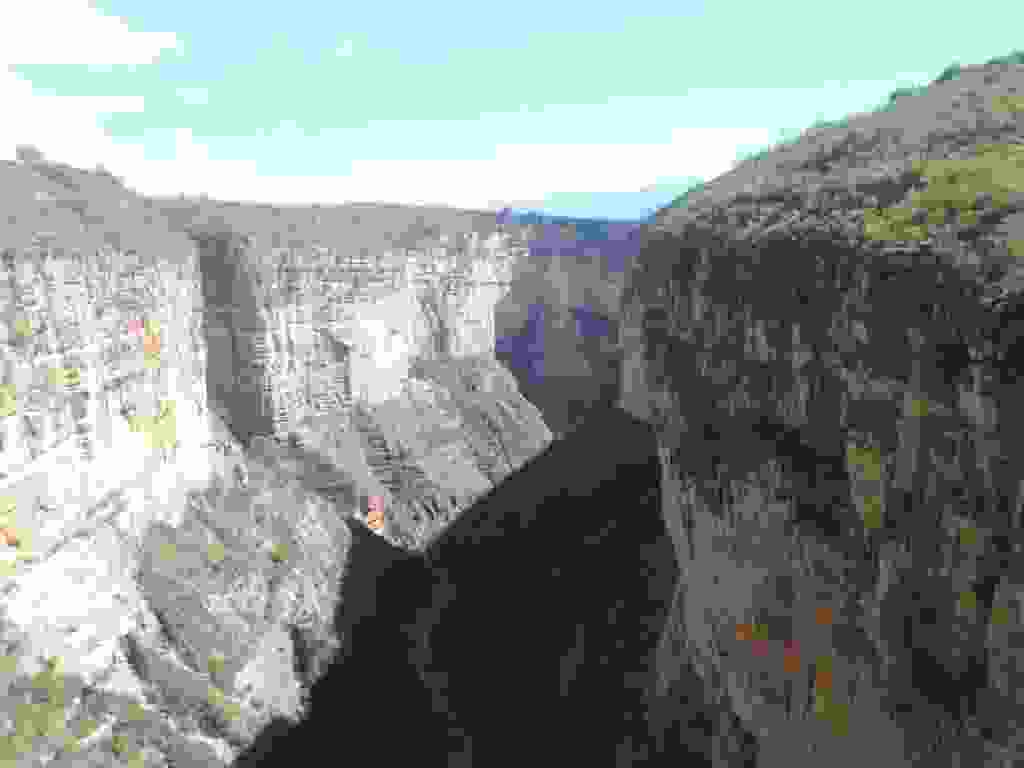
\includegraphics[height=90mm]{../wp-content/uploads/2015/04/P4263653-1024x768.jpg} } 
 \newline
 La descente au fond du canyon finit sur une belle cascade. \newline
 \newline
\centerline{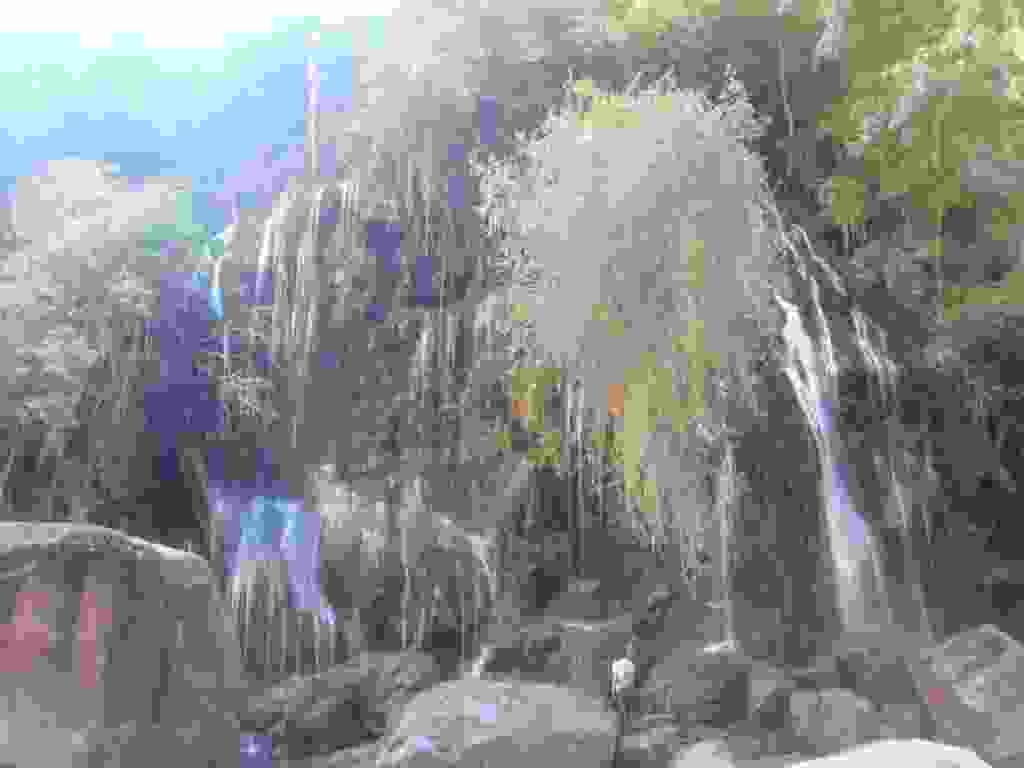
\includegraphics[height=90mm]{../wp-content/uploads/2015/04/P4263662-1024x768.jpg} } 
 \newline
 Le long du chemin, de nombreuses traces de dinosaures. \newline
 \newline
\centerline{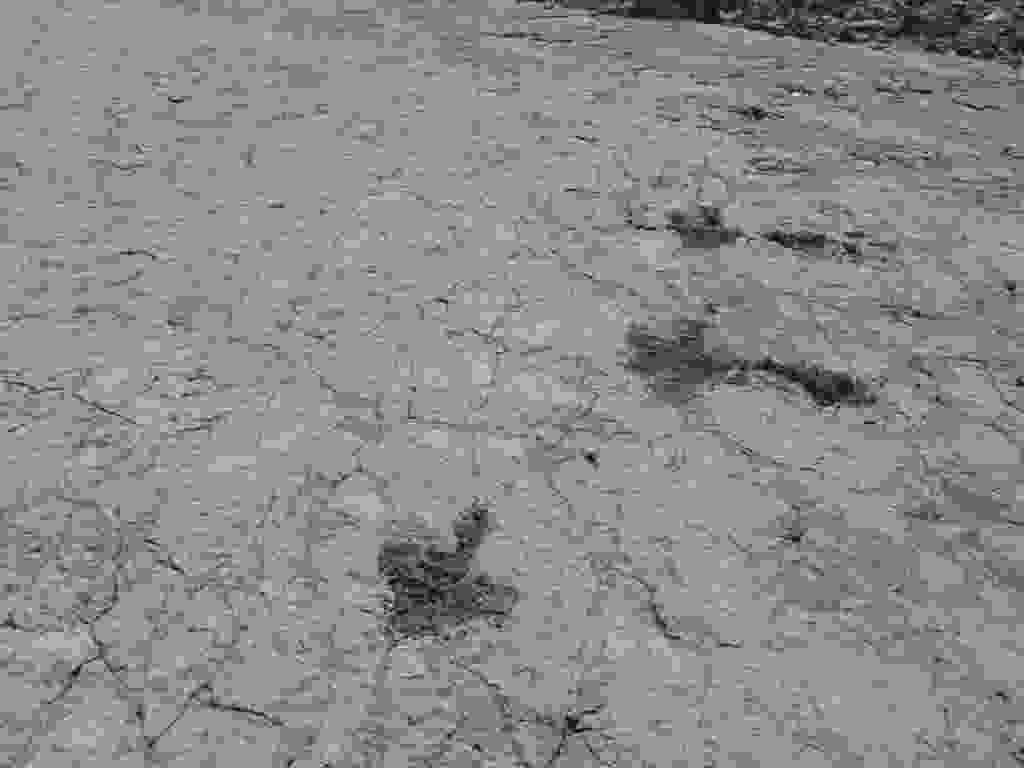
\includegraphics[height=90mm]{../wp-content/uploads/2015/04/P4253633-1024x768.jpg} } 
 \newline
 \newline
\centerline{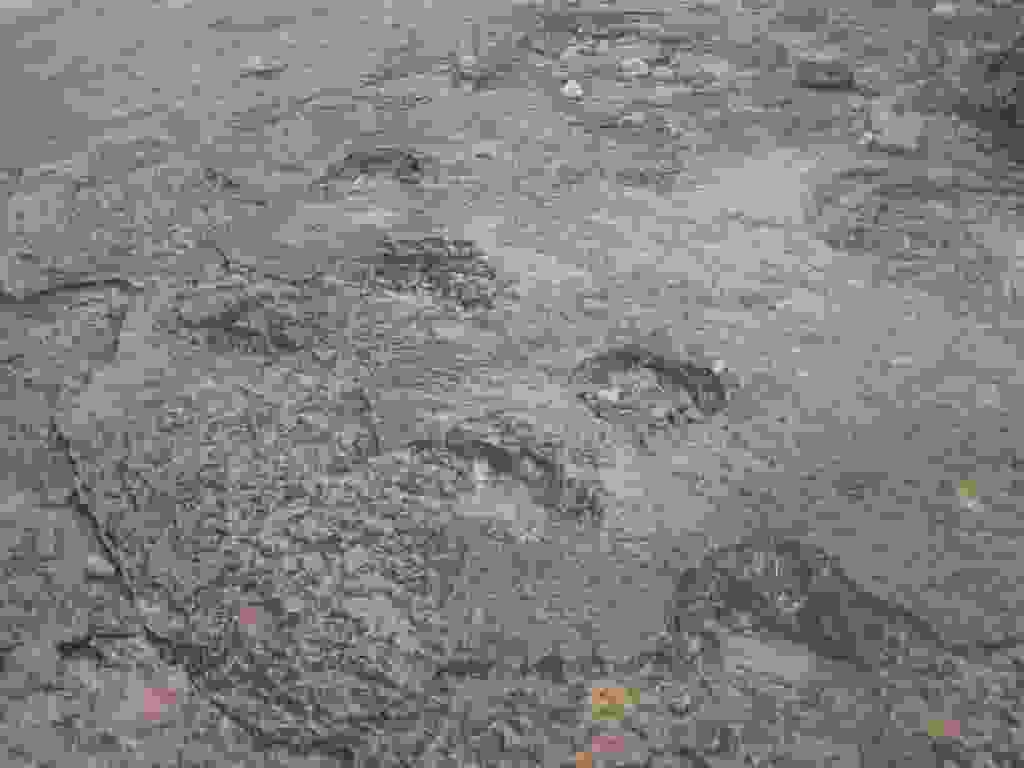
\includegraphics[height=90mm]{../wp-content/uploads/2015/04/P4263647-1024x768.jpg} } 
 \newline

\newpage
 
